\chapter{Indledning}
Flere danske hospitalsafdelinger oplever i perioder at have flere patienter end der er kapacitet til, i form af mangel på sengepladser, personale eller rum\cite{Company2013}. Overskridelsen af kapaciteten resulterer bl.a. i, at personalet får mindre tid pr. indlagt patient, hvilket kan medføre gener for både personalet og patienter.\cite{Kjeldsen2015} I budgetfordelingen for Aalborg Universitetshospital i år 2017 indgår det, at ventetiden på en operation for elektive patienter skal reduceres fra 57 dage til 50 dage\cite{Budget2016}. Dette forventes at medføre, at det daglige antal elektive patienter, der indlægges, vil skabe en reducering i antallet af ledige sengepladser til akutte patienter. 

Et estimat fra 2016 indikerer, at procentdelen af danskere over 65 år vil stige fra $29~\%$ til $34~\%$ og dermed også antallet af patienter\cite{RegionNord2016}. En stigning i antallet af patienter vil i takt med kortere ventetid på behandling skabe et aktuelt problem ift. planlægning af indlæggelser samt kapacitetudnyttelse på ortopædkirurgisk afdeling. Ifølge en undersøgelse fra Dansk Sygeplejeråd, mener hver anden regionalt ansat sygeplejerske på tværs af regionerne, at den travle arbejdsdag påvirker patientsikkerheden\cite{Kjeldsen2015}. Foruden personalets øgede risiko for at begå fejl ift. behandlingen af patienter, kan der ligeledes opstå en sundhedsrisiko ved kapacitetsmangel. Manglen på fysisk kapacitet kan give anledning til at overflytte patienter til uhensigtsmæssige områder som f.eks. hosptialsgange\cite{Madsen2014}. Dermed er der opstået et aktuelt problem som vedrører kapacitetsmangel, og konsekvenserne af dette problem bør undersøges nærmere. Ved at udnytte kapaciteten på afdelingen opnås der mere sundhed for pengene\cite{Company2013}. På baggrund af dette opstilles følgende initierende problem:\\

\noindent
\textit{Hvordan påvirkes ortopædkirurgisk afdeling på Aalborg Universitetshospital af ændringerne vedrørende kapacitetsudnyttelse og hvor udbredte er belægningsrelaterede problemer på afdelingen?}


\chapter{Problemanalyse}
\section{Kapacitet} \label{kap}
% Skriv ift kapacitet (ift sengepladser, persona - hvilken betydning har hhv. 95 \% kapacitet mod 105 \%)
Kapacitet omfatter antallet af patienter, kontakter, personale, udstyr og rum. Kontakter omfatter forundersøgelse, behandling og kontrol. Personalet består af læger, sygeplejersker og sekretærer. Udstyret beskriver de nødvendige maskiner samt antallet af rum, der opbevarer disse. Disse faktorer beskriver den samlede kapacitetsudnyttelse og er defineret ud fra, at der produceres mest muligt for de investerede ressourcer. Kapacitetudnyttelsen er forholdet mellem aktivitet og kapacitet. \cite{Company2013} En beskrivelse af dette fremgår af \figref{kapacitet}. 

\begin{figure}[H]
	\flushleft 
	\centering
	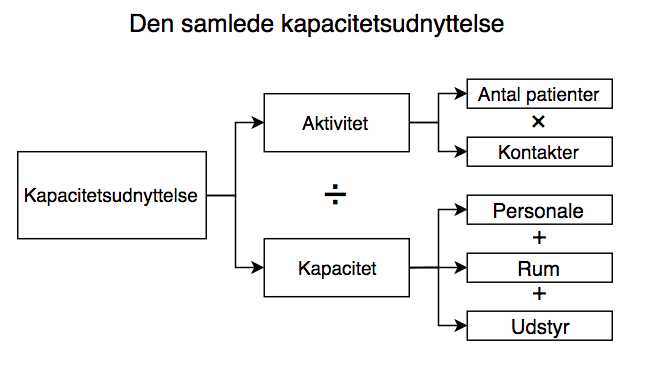
\includegraphics[scale=.45]{figures/Kapacitetsudnyttelse.png}
	\flushleft
	\caption{\textit{Opdeling af den samlede kapacitetsudnyttelse. Aktivitet omfatter af antallet patienter og kontakter. Kapacitet omfatter personale, rum og udstyr. \cite{Company2013}}}
	\label{kapacitet}
\end{figure}

\noindent
Belægning beskriver antallet af patienter, der er normeret til på en afdeling \cite{Heidmann2014}. Når en $100~\%$ belægning opnås, svarer dette til, at alle sengepladser på en afdeling er taget i brug, hvilket er fuld udnyttelse af fysisk kapacitet. Ved en belægningsgrad på over $100~\%$ betyder det, at der er flere patienter end afdelingen er normeret til, hvilket vil sige, at afdelingen yder mere end der er fysisk kapacitet til. Ved en belægningsgrad på under $100~\%$ er der omvendt færre patienter end afdelingen er normeret til, således der er tomme sengepladser og afdelingen derved ikke udnytter den fysiske kapacitet effektivt. \cite{Pauly1986} 

\section{Kapacitetsmangel}
Hvis der opstår kapacitetsmangel på ortopædkirurgisk afdeling sker der en omstrukturering af personalets arbejdsopgaver som sikre patientens behov, opretholdelse af kvalitet og udnyttelse af kompetencer. Generelt er personalet den begrænsende faktor for planlægning og kapacitetsudnyttelse\cite{Company2013}. Dette er med henblik på at finde en balance mellem de ressourcer og de krav det er i den pågældende situation. \cite{Bjerg2016} 

\subsection{Retningslinjer for personale} \label{Per_sik}
I tilfælde af ekstrem underkapacitet er der udarbejdet en arbejdstilrettelæggelse Region Nordjylland for personalet på ortopædkirurgisk afdeling. Ved kapacitetsmangel påtager lederen eller dennes stedfortræder ansvaret for at finde en løsning på dette problem. Dette kan betyde at det afgående vagthold skal blive indtil en midlertidig løsning er fundet, samt indkalde det næste vagthold tidligere. I nogle tilfælde kan det være nødvendighed at låne ressourcer fra andre afsnit eller indkalde personale fra vikarbureauet. Derudover undersøges det om behandlingen af elektive patienter kan aflyses.\cite{Bjerg2016} I tilfælde af overarbejde må en arbejdsuge for en sygeplejerske, ifølge arbejdstidsaftalen indgået med Dansk Sygeplejeråd, ikke overstige 48 timer\cite{Danske2015}.  \fxnote{Spørgsmål til sygeplejersker: Hvordan prioriteres pauser under overbelægning?} Hvis sundhedspersonalet er nødsaget til at arbejde længere end den normale arbejdstid, viser dette sig at have en negativ indvirkning på personalet.\cite{Dinges2004} Dette resulterer i en presset arbejdsdag og dermed en forringet kvalitet af behandlingen. Dertil menner hver anden regionalt ansat sygeplejerske på tværs af regionerne, at den travle arbejdsdag påvirker patienternes sikkerhed.\cite{Kjeldsen2015} 

\subsection{Patientsikkerhed}
Overflytningen af patienter bevirker til, at de oplever et skærpet privatliv. \cite{Madsen2014} Derudover kan det belaste fysiske og psykiske forhold for patienterne såvel som pårørende. \cite{Heidmann2014} Som nævnt i afsnit \ref{Per_sik} øges risikoen for fejl ved et belægningproblem og dertil ses det at mortalitetsraten øges med $1,2~\%$ ved en overskridelse af sengebelægningskapaciteten på $10~\%$ ifølge et dansk studie fra år 2014. \cite{Madsen2014} Hertil understreges det, at der kan være flere parametre, der påvirker mortaliteten og det nødvendigvis ikke er overbelægning der er den primære årsag til øget mortalitet. Overbelægning giver derfor et forøget pres for at få patienterne udskrevet, således at der opnås en normalbelægning og  den fysiske kapacitet ikke overstiges. \fxnote{Tidligere afsnit: Hvordan er fordelingen af elektive og akutte patinter? Kan elektive patienter tages ind før der er normalbelægning?} 


\section{Omfang af belægning}
På ortopædkirurgisk afdeling på Aalborg Universitetshospital ses en varierende belægningsgrad fra måned til måned. Belægningsgraden er antallet af disponible senge i brug. På \figref{maxminbelaeg} ses den varierende belægning fra år $2014$ til $2015$ på ortopædkirurgisk afdeling. \cite{SDS2015}


\begin{figure}[H]
	\flushleft 
	\centering
	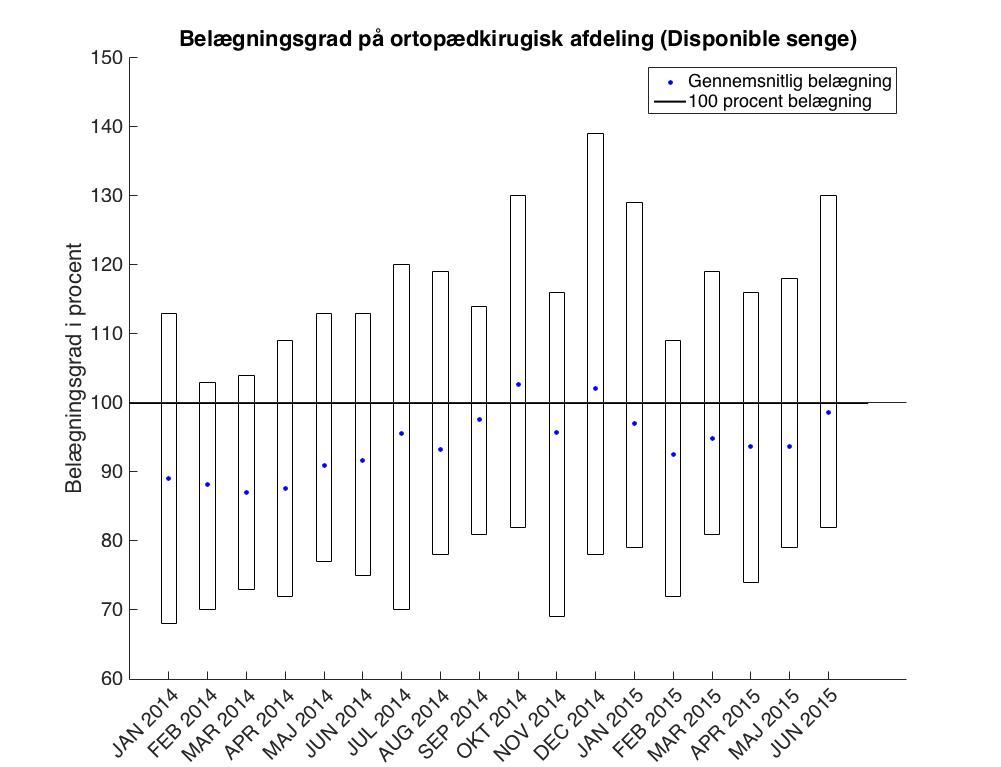
\includegraphics[scale=.40]{figures/maxminoverbelaeg.png}
	\flushleft
	\caption{\textit{Figuren illustrerer belægningsgraden over 18 måneder fra år $2014$ til $2015$ på ortopædkirurgisk afdeling på Aalborg Universitetshospital. Søjlerne viser belægning ift. $100\%$ belægning, dertil ses den gennemsnitlige belægning for hver måned som et punkt. \cite{SDS2015}}}
	\label{maxminbelaeg}
\end{figure}

\noindent
Det fremgår af \figref{maxminbelaeg}, at ortopædkirurgisk afdeling oplever en belægning hhv. over og under én ønskede belægning på $100 \%$. I december måned år $2014$ ses en maksimal belægning på $139 \%$ og en minimums belægning på $78 \%$. Dette indikerer, at ortopædkirurgisk afdeling oplever belægning over $100 \%$ i kortvarige perioder. Da \figref{maxminbelaeg} ikke viser belægningsperioden er det uvist om, hvorvidt belægningen over $100 \%$ opleves i timer eller flere dage. Der skal herudover tages forbehold for, at \figref{maxminbelaeg} både indeholder elektive samt akutte indlagte patienter, og derfor er uvist om, hvorvidt det er akutte patienter, der resulterer i en belægningsgrad på over $100 \%$. Der ses ligeledes en gennemsnitlig belægning pr. måned på \figref{maxminbelaeg}. Denne ses hyppigst under $100 \%$ belægning, hvortil der kun ses oktober samt december i år $2014$ med en gennemsnitlig belægning på over $100 \%$ belægning. Derved opleves der ikke en gennemsnitlig belægning på over $100 \%$ i $16$ ud af de $18$ oplyste måneder. \cite{SDS2015}


For at underbygge belægningsgraden yderligere, illustrerer \figref{antaldage} antal dage pr. måned med en belægningsgrad på over $100 \%$. Denne graf er udarbejdet ud fra ortopædkirurgisk afdeling over de samme 18 måneder fra år $2014$ til $2015$ som \figref{maxminbelaeg}. \cite{SDS2015} 

\begin{figure}[H]
	\flushleft 
	\centering
	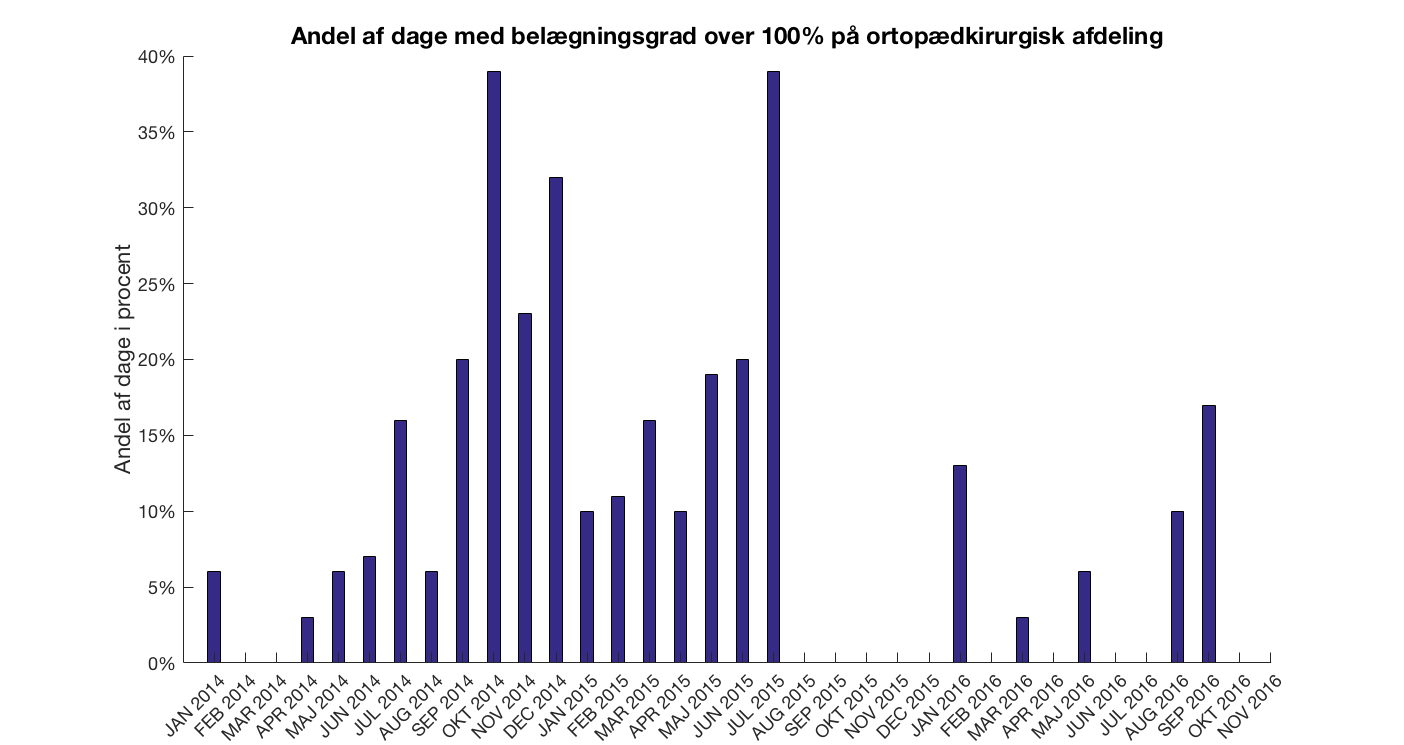
\includegraphics[scale=.4]{figures/antaldage.png}
	\flushleft
	\caption{\textit{Figuren illustrerer antal dage med en belægningsgrad over $100 \%$ fra januar 			$2014$ til juni $2015$ på ortopædkirugisk afdeling på Aalborg Universitetshospital. 					\cite{SDS2015}}}
	\label{antaldage}
\end{figure}

\noindent
Af \figref{antaldage} ses det, at der i oktober måned år 2014 opleves en belægning på over $100 \%$ i 19 dage. Det vides dog ikke, hvorvidt der er tale om én ekstra eller flere patienter, der udgør en belægningsgrad på over $100 \%$, samt hvor længe patienterne er indlagt på afdelingen. Det ses i \figref{maxminbelaeg}, at der i oktober måned år 2014 opleves en belægning på $130 \%$, hvilket kan opholdes mod de 19 dage. Det skal understreges, at begge grafer er angivet i måneder, og det er derfor uvist om, hvor mange patienter, der er indlagt pr. dag. Derudover er figurerne, \figref{maxminbelaeg} og \figref{antaldage}, udarbejdet over 18 måneder, hvilket angiveligt ikke er en repræsentativ periode for at konkludere et reelt problem på afdelingen. Dertil vides det ikke om belægningsgraden over $100 \%$ opleves som værende et problem på ortopædkirurgisk afdeling på Aalborg Universitetshospital eller om det blot er et strukturerings problem. 

\section{Problemformulering}
\textit{Hvordan kan en prædiktiv model til at forudsige indlæggelsestiden for patienter på ortopædkirurgisk afdeling på Aalborg Universitetshospital med henblik på at opretholde en kapacitet på 100 \%?}

\chapter{Fremtidige planer}
\textbf{Interview} 

Vi vil gerne foretage et interview med flere sygeplejersker på ortopædkirurgisk afdeling. Meningen med dette interview er at belyse den viden vi ikke kan finde i litteraturen. Derudover ønskes det, at gruppen besøger ortopædkirurgisk afdeling for således at observere deres arbejdsgang.  Herunder viden angående; kapacitet, kapacitetsmangel, elektive samt akutte patienter og sygeplejerskers arbejdsrutiner

Spørgsmålene er gennemgået med klinisk vejleder og AAU-vejleder inden interviewet påbegyndes. Herefter vil den kliniske vejleder kontaktes for planlægning af tidspunkt for interviewet.

Interviewet vil gentages flere gange, således gruppen får flest mulige interviews med flere sygeplejersker. Gruppen vil hertil blive opdelt, så det kun er to personer, som fører interviewet. \\

\noindent
\textbf{Problemløsning}
Vurdere forskellige prædiktive modeller og stifte bekendtskab med machine learning, samt hvilke parametre der bør anvendes.

